%%%%
%% poster.tex
%%
%% Copyright 2012 Jeffrey Finkelstein
%%
%% Except where otherwise noted, this work is made available under the terms of
%% the Creative Commons Attribution-ShareAlike 3.0 license,
%% http://creativecommons.org/licenses/by-sa/3.0/.
%%
%% You are free:
%%    * to Share — to copy, distribute and transmit the work
%%    * to Remix — to adapt the work
%% Under the following conditions:
%%    * Attribution — You must attribute the work in the manner specified by
%%    the author or licensor (but not in any way that suggests that they
%%    endorse you or your use of the work).
%%    * Share Alike — If you alter, transform, or build upon this work, you may
%%    distribute the resulting work only under the same, similar or a 
%%    compatible license.
%%    * For any reuse or distribution, you must make clear to others the 
%%    license terms of this work. The best way to do this is with a link to the
%%    web page http://creativecommons.org/licenses/by-sa/3.0/.
%%    * Any of the above conditions can be waived if you get permission from
%%    the copyright holder.
%%    * Nothing in this license impairs or restricts the author's moral rights.
%%%%
\documentclass{lposter-with-tkz-graph} % loads tkz-graph first to avoid errors

\usepackage{amsmath} % for \text{} in math mode
\usepackage{amsthm} % for theorem and definition environments
\usepackage{complexity} % for complexity class font styling
\usepackage{type1cm} % for large \mathsf fonts
\usepackage{tkz-graph} % for drawing graphs
\usepackage[matrix,arrow]{xy} % for drawing matrices with arrows

\title{Polynomial time kernel reductions}
\author{Jef{}frey Finkelstein, Ben Hescott}
\advisor{Steve Homer}
\department{Computer Science}
%\institute{Boston University}
\date{March 23}
\year{2012}

\newtheorem*{theorem}{Theorem}
\theoremstyle{definition} \newtheorem*{definition}{Definition}

\newenvironment{proofidea}{\begin{proof}[Proof idea]}{\end{proof}}

\begin{document}
\begin{poster}

%% first column

\section{A reduction for equivalence relations}
{\LARGE
\begin{figure}
  \caption{\textnormal{Polynomial time many-one reduction $f$ from $\textsf{GI}$ to $\textsf{DirGI}$.}}
  \begin{displaymath}
    \xymatrix{
      \begin{tikzpicture}[rotate=-45, scale=2]
        \GraphInit[vstyle=Normal]
        \SetGraphUnit{3}
        \SetVertexNoLabel
        \Vertices{square}{a,b,c,d}
        \Edges(c,a,b,c,d)
      \end{tikzpicture}
      & \cong & 
      \begin{tikzpicture}[rotate=-45, scale=2]
        \GraphInit[vstyle=Normal]
        \SetGraphUnit{3}
        \SetVertexNoLabel
        \Vertices{square}{a,b,c,d}
        \Edges(d,b,a,d,c)
      \end{tikzpicture}
      \\
      & \ar[dd]_f & \\
      & & \\
      & & \\
      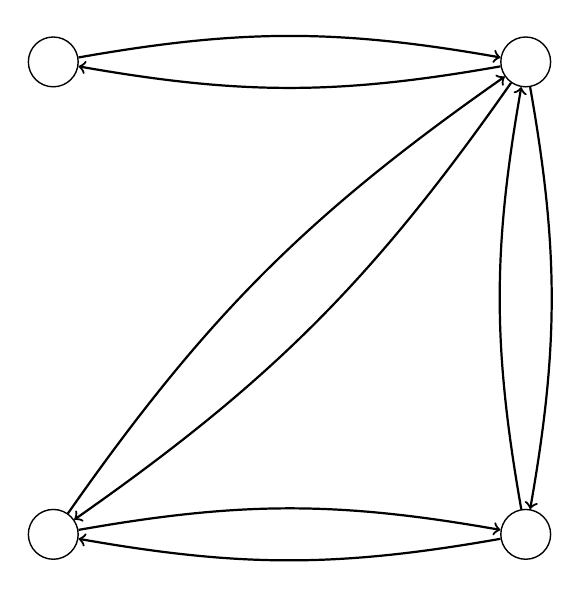
\begin{tikzpicture}[rotate=-45, scale=2]
        \GraphInit[vstyle=Normal]
        \SetGraphUnit{3}
        \SetVertexNoLabel
        \Vertices{square}{a,b,c,d}
        \Edge[style={->,bend left=10}](c)(a)
        \Edge[style={<-,bend right=10}](c)(a)
        \Edge[style={->,bend left=10}](a)(b)
        \Edge[style={<-,bend right=10}](a)(b)
        \Edge[style={->,bend left=10}](b)(c)
        \Edge[style={<-,bend right=10}](b)(c)
        \Edge[style={->,bend left=10}](c)(d)
        \Edge[style={<-,bend right=10}](c)(d)
      \end{tikzpicture}
      & \cong &
      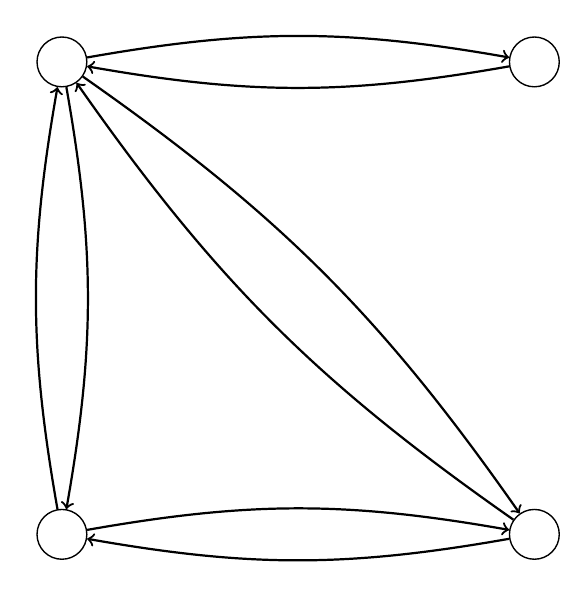
\begin{tikzpicture}[rotate=-45, scale=2]
        \GraphInit[vstyle=Normal]
        \SetGraphUnit{3}
        \SetVertexNoLabel
        \Vertices{square}{a,b,c,d}
        \Edge[style={->,bend left=10}](d)(b)
        \Edge[style={<-,bend right=10}](d)(b)
        \Edge[style={->,bend left=10}](b)(a)
        \Edge[style={<-,bend right=10}](b)(a)
        \Edge[style={->,bend left=10}](a)(d)
        \Edge[style={<-,bend right=10}](a)(d)
        \Edge[style={->,bend left=10}](d)(c)
        \Edge[style={<-,bend right=10}](d)(c)
      \end{tikzpicture}
  }
  \end{displaymath}
\end{figure}

\begin{figure}
  \caption{\textnormal{Polynomial time kernel reduction $g$ from $\textsf{GI}$ to $\textsf{DirGI}$.}}
  \begin{displaymath}
    \xymatrix{
      \begin{tikzpicture}[rotate=-45, scale=2]
        \GraphInit[vstyle=Normal]
        \SetGraphUnit{3}
        \SetVertexNoLabel
        \Vertices{square}{a,b,c,d}
        \Edges(c,a,b,c,d)
      \end{tikzpicture}
      \ar[ddd]_g & \cong & 
      \begin{tikzpicture}[rotate=-45, scale=2]
        \GraphInit[vstyle=Normal]
        \SetGraphUnit{3}
        \SetVertexNoLabel
        \Vertices{square}{a,b,c,d}
        \Edges(d,b,a,d,c)
      \end{tikzpicture}
      \ar[ddd]_g \\
      & & \\
      & & \\
      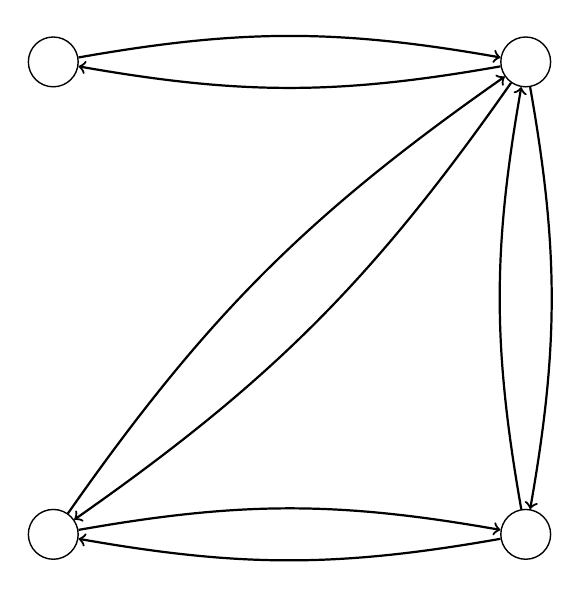
\begin{tikzpicture}[rotate=-45, scale=2]
        \GraphInit[vstyle=Normal]
        \SetGraphUnit{3}
        \SetVertexNoLabel
        \Vertices{square}{a,b,c,d}
        \Edge[style={->,bend left=10}](c)(a)
        \Edge[style={<-,bend right=10}](c)(a)
        \Edge[style={->,bend left=10}](a)(b)
        \Edge[style={<-,bend right=10}](a)(b)
        \Edge[style={->,bend left=10}](b)(c)
        \Edge[style={<-,bend right=10}](b)(c)
        \Edge[style={->,bend left=10}](c)(d)
        \Edge[style={<-,bend right=10}](c)(d)
      \end{tikzpicture}
      & \cong &
      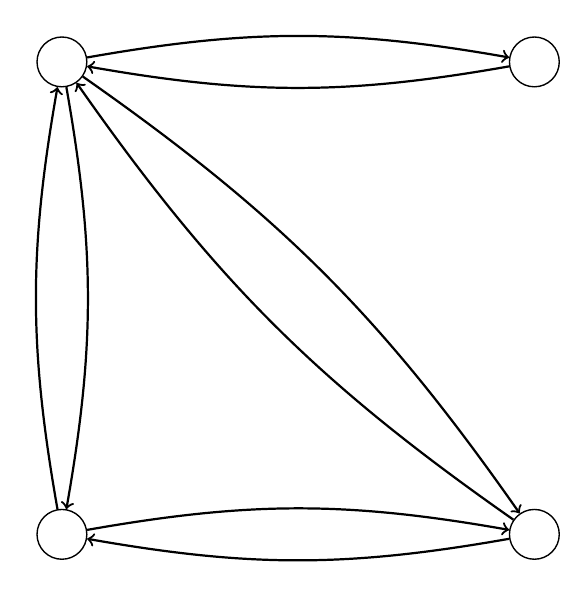
\begin{tikzpicture}[rotate=-45, scale=2]
        \GraphInit[vstyle=Normal]
        \SetGraphUnit{3}
        \SetVertexNoLabel
        \Vertices{square}{a,b,c,d}
        \Edge[style={->,bend left=10}](d)(b)
        \Edge[style={<-,bend right=10}](d)(b)
        \Edge[style={->,bend left=10}](b)(a)
        \Edge[style={<-,bend right=10}](b)(a)
        \Edge[style={->,bend left=10}](a)(d)
        \Edge[style={<-,bend right=10}](a)(d)
        \Edge[style={->,bend left=10}](d)(c)
        \Edge[style={<-,bend right=10}](d)(c)
      \end{tikzpicture}
  }
  \end{displaymath}
\end{figure}
}


\columnbreak

%% second column

{\setlength{\parindent}{0cm}\textbf{\large A study of the power of polynomial time kernel reductions among problems of equivalence.}}

\vspace{0.5cm}

\begin{definition}
  If $R$ and $S$ are equivalence relations, $R$ \emph{polynomial time kernel reduces to} $S$ if there exists a polynomial time computable function $f$ such that for all $x$ and $y$,
  \begin{displaymath}
    (x, y)\in R \iff (f(x), f(y))\in S.
  \end{displaymath}
\end{definition}

\vspace{0.5cm}

\begin{definition}\mbox{}
  \begin{itemize}
    \renewcommand{\labelitemi}{$\cdot$}
  \item $\PEq$: equivalence problems in $\P$
  \item $\NPEq$: equivalence problems in $\NP$
  \item $\SKPEq$: equivalence problems in $\SKP$
  \item $\PKPEq$: equivalence problems in $\PKP$
  \item $\PSPACEEq$: equivalence problems in $\PSPACE$
  \end{itemize}
\end{definition}


\section{Hard problems under kernel reductions}
\newcommand{\indentitem}{\setlength\itemindent{1cm}}
\begin{theorem}
  Under polynomial time kernel reductions,
  \begin{enumerate}
  {\indentitem \item $\PSPACEEq$ has a complete problem}
  {\indentitem \item $\PKPOPEq$ contains a problem which is hard for $\SKPEq$, for all $k\geq 0$}
  {\indentitem \item $\PKPOPEq$ contains a problem which is hard for $\PKPEq$, for all $k\geq 0$}
  \end{enumerate}
\end{theorem}

\begin{proofidea}
  Turn the canonical complete problem for $\NP$,
  \begin{displaymath}
    K = \left\{(M, x, 1^t)\,\middle|\,M\text{ accepts } x \text{ within } t \text{ steps}\right\},
  \end{displaymath}
  into an equivalence relation, $R_K$, which relies on the hardness of $K$.
  Use a helper algorithm to enforce that the language of the machine $M$ is an equivalence relation (for strings up to a certain length).
  This helper algorithm bumps up the hardness of the problem to the next level of the polynomial time hierarchy.
\end{proofidea}


\section{Sizes of equivalence classes matter}
\begin{theorem}
  If the number of equivalence classes of $R$ is superpolynomial and the number of equivalence classes of $S$ is polynomial, then $R$ does not polynomial time kernel reduce to $S$.
\end{theorem}
\vspace{1cm}
\begin{proofidea}
  All elements of a single equivalence class of $R$ must have images which are in the same equivalence class of $S$.
  If such a kernel reduction were to exist, the pigeonhole principle would force elements from two different equivalence classes of $R$ to be mapped to a single equivalence class of $S$.
\end{proofidea}


\columnbreak

%% third column

\section{Intermediary problems}
%%%%
%% intermediary.tex
%%
%% Copyright 2011 Jeffrey Finkelstein
%%
%% Except where otherwise noted, this work is made available under the terms of
%% the Creative Commons Attribution-ShareAlike 3.0 license,
%% http://creativecommons.org/licenses/by-sa/3.0/.
%%
%% You are free:
%%    * to Share — to copy, distribute and transmit the work
%%    * to Remix — to adapt the work
%% Under the following conditions:
%%    * Attribution — You must attribute the work in the manner specified by
%%    the author or licensor (but not in any way that suggests that they
%%    endorse you or your use of the work).
%%    * Share Alike — If you alter, transform, or build upon this work, you may
%%    distribute the resulting work only under the same, similar or a 
%%    compatible license.
%%    * For any reuse or distribution, you must make clear to others the 
%%    license terms of this work. The best way to do this is with a link to the
%%    web page http://creativecommons.org/licenses/by-sa/3.0/.
%%    * Any of the above conditions can be waived if you get permission from
%%    the copyright holder.
%%    * Nothing in this license impairs or restricts the author's moral rights.
%%%%
\section{Existence of intermediary problems}

We will denote by $\NPEqC$ the set of equivalence relations which are $\kr$-complete for \NPEq.

The main result of this section is as follows.
\begin{reptheorem}{thm:intermediary}
  \printintermediarytheorem
\end{reptheorem}
To show this, we will adapt a proof of Ladner's original theorem\cite{ladner} showing that if $\P\neq\NP$ then there exist problems in $\NP$ which are neither in $\P$ nor \NP-complete.
The proof we follow can be found in \cite{bdg95}, which is an adaptation of Sch\"{o}ning's proof of the ``uniform diagonalization theorem''\cite{schoning}, which is itself a generalization of Ladner's original method.

First we need to provide some technical definitions and machinery.

\begin{definition}
  A class of languages $\mathcal{C}$ is \defn{closed under finite variations} if and only if $A\in \mathcal{C}$ and $A\symdiff B$ (the symmetric difference of $A$ and $B$) is finite implies $B\in \mathcal{C}$ for all $B$.
\end{definition}

\begin{definition}
  Given an alphabet $\Sigma$ with at least two different symbols, say $0$ and $1$, the \defn{kernel join} of two equivalence relations $R$ and $S$ over $\Sigma^*$ is $R\kj S=\{\pair{x0}{y0}|\pair{x}{y}\in R\}\cup\{\pair{x1}{y1}|\pair{x}{y}\in S\}$.
\end{definition}

\begin{lemma}\label{lem:join}
  If $R$ and $S$ are equivalence relations on $\Sigma^*$, then $R\kj S$ is an equivalence relation (on $\Sigma^*\backslash\{\lambda\}$).
\end{lemma}
\begin{proof}
  Let $x$, $y$ and $z$ be non-empty strings in $\Sigma^*$.
  
  Since $x$ is non-empty, $x=x'0$ or $x=x'1$.
  Since $R$ is reflexive, $\pair{x'}{x'}\in R$.
  Hence $\pair{x}{x}\in R\kj S$.
  Therefore $R\kj S$ is reflexive.
  
  Suppose $\pair{x}{y}\in R\kj S$.
  Then either $x=x'0$, $y=y'0$ and $\pair{x'}{y'}\in R$ or $x=x'1$, $y=y'1$ and $\pair{x'}{y'}\in S$.
  In either case, symmetry follows from the symmetry of $R$ or $S$.

  Suppose $\pair{x}{y}$ and $\pair{y}{z}$ are both in $R\kj S$.
  In the case that $x=x'0$, $y=y'0$ and $\pair{x'}{y'}\in R$, and that $z=z'0$ and $\pair{y'}{z'}\in R$, then by the transitivity of $R$, $\pair{x'}{z'}\in R$, so $\pair{x}{z}\in R\kj S$.
  The argument is similar in the case that $x=x'1$, $y=y'1$ and $z=z'1$.
  It is a contradiction for the other two cases to exist, since $y$ cannot be equal to both $y'0$ and $y'1$.

  Since $R\kj S$ is reflexive, symmetric and transitive, $R\kj S$ is an equivalence relation.
\end{proof}

\begin{proposition}\label{prop:symdiff}
  Symmetric difference of equivalence relations preserves symmetry.
\end{proposition}
\begin{proof}
  Let $R$ and $S$ be equivalence relations.
  Let $(x,y)\in(R\symdiff S)$.
  In the case that $(x,y)\in R$ and $(x,y)\notin S$, then $(y,x)\in R$.
  If $(y,x)$ were in $S$, then $(x,y)$ would also be in $S$, by symmetry, but this is a contradiction.
  Hence $(y,x)\in R$ and $(y,x)\notin S$.
  The argument for the other case is symmetric.
  Therefore $(x,y)\in(R\symdiff S)\implies (y,x)\in(R\symdiff S)$.
\end{proof}

\begin{definition}
  Let $r\colon\mathbb{N}\to\mathbb{N}$ be a computable function such that $r(m)>m$ for all $m$.
  Define the set $G[r]$ as
  \begin{displaymath}
    G[r]=\{x\in\Sigma^*|r^n(0)\leq|x|<r^{n+1}(0) \plain{for some even} n\}
  \end{displaymath}
  where $r^n(m)$ denotes the $n$-fold application of $r$ to $m$:
  \begin{displaymath}
    \overbrace{r\circ r\circ r\circ\cdots\circ r}^{n \plain{times}}(m)
  \end{displaymath}
  $G[r]$ is called the \defn{gap language} generated by $r$.
\end{definition}

\begin{lemma}\label{lem:gap_p}
  If $r$ is time constructible, then $G[r]\in\P$.
\end{lemma}
\begin{proof}
  Proof omitted.
\end{proof}

We will denote the Cartesian product $G[r]\times G[r]$ by the slightly more succinct ${G[r]}^2$, and $\overline{G[r]}\times\overline{G[r]}$ by $\overline{G[r]}^2$.
Elements of ${G[r]}^2$ are pairs of strings whose lengths are in the ``even gaps'' of $r$, while elements of $\overline{G[r]}^2$ are pairs of strings whose lengths are in the ``odd gaps'' of $r$.

\begin{lemma}
  ${G[r]}^2$ and $\overline{G[r]}^2$ are \defn{partial equivalence relations} (that is, they are symmetric and transitive).
\end{lemma}
\begin{proof}
  We will prove the theorem for ${G[r]}^2$; a symmetric argument proves the theorem for $\overline{G[r]}^2$.

  Let $x,y\in\Sigma^*$.
  Suppose $\pair{x}{y}\in {G[r]}^2$, so the lengths of $x$ and $y$ are both in an even gap of $r$.
  Then $\pair{y}{x}\in{G[r]}^2$, so ${G[r]}^2$ is symmetric.
  Now let $z\in\Sigma^*$ and suppose also that $\pair{y}{z}\in {G[r]}^2$.
  Then $y$ and $z$ are both in an even gap of $r$, so $x$, $y$ and $z$ are all in some even gap of $r$, and hence $\pair{x}{z}\in {G[r]}^2$.
  Therefore ${G[r]}^2$ is transitive.
\end{proof}

We are now prepared to prove the main technical theorem which will allow us to construct an equivalence relation which is ``between'' two complexity classes.

\begin{theorem}\label{thm:diag}
  Let $R_1$ and $R_2$ be decidable equivalence relations, and let $\mathcal{C}_1$ and $\mathcal{C}_2$ be classes of decidable equivalence relations such that:
  \begin{enumerate}
  \item $R_1\notin\mathcal{C}_1$
  \item $R_2\notin\mathcal{C}_2$
  \item $\mathcal{C}_1$ and $\mathcal{C}_2$ are computably enumerable
  \item $\mathcal{C}_1$ and $\mathcal{C}_2$ are closed under finite variations
  \end{enumerate}
  Then there exists a decidable equivalence relation $R$ such that:
  \begin{enumerate}
  \item $R\notin \mathcal{C}_1$
  \item $R\notin \mathcal{C}_2$
  \item $R\kr R_1\kj R_2$
  \end{enumerate}
\end{theorem}
\begin{proof}
  Let $P_1, P_2, \ldots$ and $Q_1, Q_2, \ldots$ be enumerations of Turing machines deciding the languages in $\mathcal{C}_1$ and $\mathcal{C}_2$ respectively.
  Define the functions
  \begin{eqnarray*}
    r_1(n)=\underset{i\leq n}{max}\{|z_{i,n}|\}+1 & \text{and} &
    r_2(n)=\underset{i\leq n}{max}\{|z'_{i,n}|\}+1
  \end{eqnarray*}
  where $z_{i,n}$ is the smallest word in $\Sigma^*$ such that there exists an $x\in\Sigma^*$, with $n<|x|\leq|z_{i,n}|$, such that $\pair{z_{i,n}}{x}\in(L(P_i)\symdiff R_1)$, and $z'_{i,n}$ is the smallest word in $\Sigma^*$ such that there exists an $x'\in\Sigma^*$, with $n<|x'|\leq|z'_{i,n}|$, such that $\pair{z'_{i,n}}{x'}\in(L(Q_i)\symdiff R_2)$.
  Note that it also suffices to find an $x$ and $x'$ such that $\pair{x}{z_{i,n}}\in(L(P_i)\symdiff R_1)$ and $\pair{x'}{z'_{i,n}}\in(L(Q_i)\symdiff R_2)$, since symmetric difference on equivalence relations preserves symmetry by \autoref{prop:symdiff}.
  The more important requirement is that $|x|\leq|z_{i,n}|$, since we will require below that both $x$ and $z_{i,n}$ are in the same gap of a specific function.

  We claim that $z_{i,n}$ and $z'_{i,n}$ always exist.
  Assume that no such $z_{i,n}$ exists, so there are no words such that there exists an $x\in\Sigma^*$, with $n<|x|\leq|z_{i,n}|$, such that $\pair{z_{i,n}}{x}\in(L(P_i)\symdiff R_1)$.
  Therefore, there are no pairs in $(L(P_i)\symdiff R_1)$ with both elements of length greater than $n$.
  Then there are a finite number of pairs in $L(P_i)\symdiff R_1$, so $R_1$ is a finite variation of $L(P_i)$.
  Since $\mathcal{C}_1$ is closed under finite variations, $R_1\in\mathcal{C}_1$.
  This is a contradiction with the hypothesis that $R_1\notin\mathcal{C}_1$.
  Therefore such a $z_{i,n}$ always exists.
  The argument that $z'_{i,n}$ always exists is similar.

  Since $L(P_i)$ and $L(Q_i)$ are decidable for all $i$, and since $R_1$ and $R_2$ are decidable, so are $L(P_i)\symdiff R_1$ and $L(Q_i)\symdiff R_2$.
  For each $n$, there is a procedure which always halts and which computes $z_{i,n}$.
  A similar procedure computes $z'_{i,n}$.
  The procedure which computes the maximum of a finite set of numbers and which adds one to that value always halts as well, so $r_1$ and $r_2$ are total computable functions.

  Let $r\ge \max(r_1,r_2)$ be a non-decreasing time constructible function, which exists by \autoref{lem:nondec}.
  Now for all $n$ and all $i\leq n$, each element of the pair $\pair{z_{i,n}}{x}$ has length between $n$ and $r_1(n)$, by construction.
  The same is true for $\pair{z'_{i,n}}{x'}$ between $n$ and $r_2(n)$.
  Notice that $\pair{z_{i,n}}{x}$ and $\pair{z'_{i,n}}{x'}$ are ``witnesses'' that $R_1\neq L(P_i)$ and $R_2\neq L(Q_i)$ respectively.
  Hence for all $n$, there are some witnesses between $n$ and $r(n)$ that for all $i\leq n$, $R_1\neq L(P_i)$ and $R_2\neq L(Q_i)$.

  Define $R=({G[r]}^2\cap R_1)\cup(\overline{G[r]}^2\cap R_2)$, so $R$ is equal to pairs of $R_1$ in the ``even gaps'' of r and $R$ is equal to pairs of $R_2$ in the ``odd gaps'' of $r$.
  It remains to show that $R$ is an equivalence relation which satisfies the properties stated in the theorem.

  First we show that $R$ is indeed an equivalence relation.
  Symmetry and transitivity follow from the symmetry and transitivity of $R_1$, $R_2$, ${G[r]}^2$ and $\overline{G[r]}^2$.
  To show reflexivity, suppose $x\in G[r]$.
  Hence $\pair{x}{x}\in {G[r]}^2$.
  Since $R_1$ is an equivalence relation, $\pair{x}{x}\in R_1$.
  Therefore $\pair{x}{x}\in({G[r]}^2\cap R_1)$, so $\pair{x}{x}\in R$.
  The argument for the case that $x\in\overline{G[r]}$ is similar.
  Therefore $R$ is reflexive, symmetric and transitive.

  Next we show that $R\notin\mathcal{C}_1$.
  The argument which proves $R\notin\mathcal{C}_2$ is symmetric.
  Assume $R\in\mathcal{C}_1$ in order to produce a contradiction.
  Then there exists an $i$ such that $R=L(P_i)$.
  Let $m$ be an even integer such that $r^m(0)\geq i$.
  By construction, there exists a pair $\pair{x}{z}$ such that $r^m(0)\leq|x|\leq|z|<r^{m+1}(0)$ and $\pair{x}{z}\in(L(P_i)\symdiff R_1)$.
  Since $m$ is even, $\pair{x}{z}\in {G[r]}^2$.
  Since $R$ is equal to $R_1$ where it coincides with ${G[r]}^2$, then $\pair{x}{z}\in(L(P_i)\symdiff R)$.
  This is a contradiction with the hypothesis that $R=L(P_i)$.
  Therefore $R\notin\mathcal{C}_1$.

  Finally, we show that $R\kr R_1\kj R_2$.
  First, we note that $R_1\kj R_2$ is an equivalence relation by \autoref{lem:join}, so a kernel reduction here is syntactically possible.
  Since $G[r]\in\P$ by \autoref{lem:gap_p}, the function defined by
  \begin{displaymath}
    f(x)=
    \begin{cases}
      x0 & \text{if}\, x\in G[r]\\
      x1 & \text{if}\, x\notin G[r]\\
    \end{cases}
  \end{displaymath}
  is a polynomial time computable function.
  
  To show that $f$ computes the reduction from $R$ to $R_1\kj R_2$ correctly, suppose first that $\pair{x}{y}\in R$, so $\pair{x}{y}$ is in either $({G[r]}^2\cap R_1)$ or $\overline{G[r]}^2\cap R_2)$.
  In the former case, both $x$ and $y$ are in $G[r]$, so $f(x)=x0$ and $f(y)=y0$, and both $x$ and $y$ are in $R_1$, so $\pair{x0}{y0}=\pair{f(x)}{f(y)}\in R_1$.
  The argument for the latter case is symmetric.

  For the converse, suppose $\pair{f(x)}{f(y)}\in R_1\kj R_2$.
  Then $f(x)$ and $f(y)$ either both end with $0$ or both end with $1$.
  In the case that both end with $0$, then there exist some strings $w_x$ and $w_y$ such that $f(x)=w_x0$, $f(y)=w_y0$ and $\pair{w_x}{w_y}\in R_1$.
  By construction of $f$, $w_x$ must equal the input $x$ and $w_y$ must equal the input $y$, so $\pair{x}{y}\in R_1$.
  Also by construction, $f(x)=x0$ if and only if $x\in G[x]$ and $f(y)=y0$ if and only if $y\in G[x]$, so $\pair{x}{y}\in{G[r]}^2$.
  Hence $\pair{x}{y}\in({G[r]}^2\cap R_1\subseteq R$.
  The argument for the case that both $f(x)$ and $f(y)$ end with $1$ is symmetric, and shows that $\pair{x}{y}\in(\overline{G[r]}^2\cap R_2)\subseteq R$.
  Therefore $\pair{x}{y}\in R$ if and only if $\pair{f(x)}{f(y)}\in R_1\kj R_2$, so $f$ correctly computes the reduction from $R$ to $R_1\kj R_2$.

  Since we have shown that the equivalence relation $R$ satisfies the properties in the statement of the theorem, this concludes the proof.
\end{proof}

We would now like to show that the result of this theorem holds when $\mathcal{C}_1=\PEq$ and $\mathcal{C}_2=\NPEqC$.

\begin{proposition}
  \mbox{} % to put the next item on a new line
  \begin{enumerate}
  \item $\PEq$ is computably enumerable.
  \item $\NPEqC$ is computably enumerable.
  \end{enumerate}
\end{proposition}
\begin{proof}
  These statements are true since any subset of a computably enumerable set is computably enumerable, and these are both subsets of $\NP$.
  Note that $\NPEqC$ may be empty.
\end{proof}

\begin{proposition}\label{prop:npeqc}
  If $\PEq\neq\NPEq$ and $\NPEqC$ is non-empty, then $\PEq\cap\NPEqC=\emptyset$.
\end{proposition}
\begin{proof}
  Assume $\PEq\cap\NPEqC\neq\emptyset$.
  Let $R$ be the \NPEq-complete equivalence relation which is also in \PEq.
  Then all problems can be kernel reduced to $R$ in polynomial time, and $R$ can be decided in polynomial time.
  Therefore, $\PEq=\NPEq$.
  This is a contradiction with the hypothesis.
  Therefore $\PEq\cap\NPEqC=\emptyset$.
\end{proof}

\begin{theorem}\label{thm:intermediary}
  \printintermediarytheorem
\end{theorem}
\begin{proof}
  The hypothesis of this theorem is the same as in \autoref{prop:npeqc}, so $\PEq\cap\NPEqC=\emptyset$.
  Let $S$ be an \NPEq-complete problem.
  Choose $R_1=S$, $R_2=\emptyset$, $\mathcal{C}_1=\PEq$ and $\mathcal{C}_2=\NPEqC$.
  Then by \autoref{thm:diag}, there exists an equivalence relation $R$ which is in neither $\NPEqC$ nor $\PEq$, but which kernel reduces to $S\kj\emptyset$.
  Since $S\kj\emptyset$ trivially kernel reduces to $S$, and since polynomial time kernel reductions compose by \autoref{prop:compose}, $R\kr S$.
  Since $\NPEq$ is closed under polynomial time kernel reductions by \autoref{prop:closed_under_kr}, $R\in\NPEq$.
\end{proof}


\section{Further work}
\begin{itemize}
  \renewcommand{\labelitemi}{$\cdot$}
\item Are there natural $\PSPACEEq$-complete problems?
\item Do existing complexity results concerning problems of equivalence using many-one reductions hold when using kernel reductions?
\item Under what general conditions does a complexity class have a complete problem under kernel reductions?
\item Can we construct problems which are hard under polynomial time kernel reductions for smaller or larger complexity classes?
\item \textbf{Does $\NPEq$ have a complete problem?}
\end{itemize}


\nocite{bcffm}
\nocite{fg09}
\bibliographystyle{plain}
\bibliography{references}

%\section{About this work}
%%%%%
%% about.tex
%%
%% Copyright 2012 Jeffrey Finkelstein
%%
%% Except where otherwise noted, this work is made available under the terms of
%% the Creative Commons Attribution-ShareAlike 3.0 license,
%% http://creativecommons.org/licenses/by-sa/3.0/.
%%
%% You are free:
%%    * to Share — to copy, distribute and transmit the work
%%    * to Remix — to adapt the work
%% Under the following conditions:
%%    * Attribution — You must attribute the work in the manner specified by
%%    the author or licensor (but not in any way that suggests that they
%%    endorse you or your use of the work).
%%    * Share Alike — If you alter, transform, or build upon this work, you may
%%    distribute the resulting work only under the same, similar or a 
%%    compatible license.
%%    * For any reuse or distribution, you must make clear to others the 
%%    license terms of this work. The best way to do this is with a link to the
%%    web page http://creativecommons.org/licenses/by-sa/3.0/.
%%    * Any of the above conditions can be waived if you get permission from
%%    the copyright holder.
%%    * Nothing in this license impairs or restricts the author's moral rights.
%%%%
\section{About this work}

This work is licensed under the Creative Commons Attribution-ShareAlike License.
Visit \mbox{\url{https://creativecommons.org/licenses/by-sa/3.0/}} to view a copy of this license.

The \LaTeX{} markup which generated this document is available at \mbox{\url{https://github.com/jfinkels/equivalence}}.
It is also licensed under the Creative Commons Attribution-ShareAlike License.

The authors can be contacted via email at \email{jeffreyf@bu.edu} and \email{hescott@cs.tufts.edu}.


\end{poster}
\end{document}
